\documentclass[11pt,border=2pt]{standalone}
% Estilo comum das figuras. Cada figura e um arquivo standalone que carrega
% este preambulo; a fonte e o corpo sao os do texto (Latin Modern, 11pt).
\usepackage[utf8]{inputenc}
\usepackage[T1]{fontenc}
\usepackage{lmodern}
\usepackage{pgfplots}
\usepackage{pgfplotstable}
\usepgfplotslibrary{groupplots}
\usetikzlibrary{calc}
\pgfplotsset{compat=1.17}

\definecolor{cg1}{RGB}{27,54,93}     % alta portabilidade
\definecolor{cg2}{RGB}{125,125,125}  % media
\definecolor{cg3}{RGB}{192,86,33}    % baixa
\definecolor{faixa}{RGB}{236,236,236}
\colorlet{faixarec}{cg3!20}
\colorlet{faixapan}{cg1!16}
\definecolor{v1}{RGB}{166,64,20}
\definecolor{v2}{RGB}{222,134,84}
\definecolor{v3}{RGB}{245,208,180}
\definecolor{v4}{RGB}{183,198,219}
\definecolor{v5}{RGB}{52,88,138}
\definecolor{c1}{RGB}{228,234,242}
\definecolor{c2}{RGB}{183,198,219}
\definecolor{c3}{RGB}{127,153,189}
\definecolor{c4}{RGB}{69,106,154}
\definecolor{c5}{RGB}{27,54,93}

\pgfplotsset{
  every axis/.append style={
    font=\footnotesize,
    axis x line*=bottom,
    axis y line*=left,
    axis line style={line width=0.4pt},
    tick align=outside,
    tick style={line width=0.4pt, black},
    major tick length=2.5pt,
    /pgf/number format/1000 sep={},
    legend style={draw=none, fill=none, font=\footnotesize,
                  legend cell align=left, /tikz/every even column/.append style={column sep=8pt}},
    title style={font=\footnotesize, yshift=-3pt},
    label style={font=\footnotesize},
    clip=false,
    scaled ticks=false,
  },
}
\tikzset{
  g1/.style={cg1, line width=0.95pt},
  g2/.style={cg2, line width=0.8pt, densely dashed},
  g3/.style={cg3, line width=0.95pt},
  fino/.style={black, line width=0.3pt},
  ufborda/.style={draw=black!75, line width=0.25pt, line join=round},
  csem/.style={fill=black!6, draw=white, line width=0.12pt},
  v1/.style={fill=v1, draw=white, line width=0.12pt, even odd rule},
  v2/.style={fill=v2, draw=white, line width=0.12pt, even odd rule},
  v3/.style={fill=v3, draw=white, line width=0.12pt, even odd rule},
  v4/.style={fill=v4, draw=white, line width=0.12pt, even odd rule},
  v5/.style={fill=v5, draw=white, line width=0.12pt, even odd rule},
  c1/.style={fill=c1, draw=white, line width=0.12pt, even odd rule},
  c2/.style={fill=c2, draw=white, line width=0.12pt, even odd rule},
  c3/.style={fill=c3, draw=white, line width=0.12pt, even odd rule},
  c4/.style={fill=c4, draw=white, line width=0.12pt, even odd rule},
  c5/.style={fill=c5, draw=white, line width=0.12pt, even odd rule},
}
% faixas coloridas do grafico de contexto
\newcommand{\dados}[1]{dados/#1.dat}

% faixas das duas crises. Em series anuais o ponto do ano t fica em t.
\newcommand{\crises}[2]{%
  \fill[faixa] (axis cs:2014.5,#1) rectangle (axis cs:2016.5,#2);
  \fill[faixa] (axis cs:2019.5,#1) rectangle (axis cs:2021.5,#2);}
% legenda de classes dos mapas: \legmapa{nome}{prefixo de cor}{x inicial}{passo}
\newcommand{\legmapa}[4]{%
  \foreach \l [count=\i from 0] in {a,b,c,d,e} {
    \pgfmathtruncatemacro{\n}{\i+1}
    \fill[#2\n, draw=none] (#3+\i*#4,-0.45) rectangle +(0.32,0.2);
    \node[font=\scriptsize, anchor=west] at (#3+0.35+\i*#4,-0.35) {\csname leg#1\l\endcsname};
  }}

% legenda vertical no canto inferior esquerdo do mapa: \legmapav{nome}{prefixo de cor}
\newcommand{\legmapav}[2]{%
  \foreach \l [count=\i from 0] in {e,d,c,b,a} {
    \pgfmathtruncatemacro{\n}{5-\i}
    \fill[#2\n, draw=none] (0.05,2.25-\i*0.36) rectangle +(0.32,0.22);
    \node[font=\scriptsize, anchor=west] at (0.42,2.36-\i*0.36) {\csname leg#1\l\endcsname};
  }}

\usetikzlibrary{arrows.meta, calc}
% Fluxograma: construcao das coortes e desfechos observados (seis coortes somadas).
% Selecao: saidas/dados/transicoes_amostra.csv (pessoas, uma_demissao,
% sem_outro_emprego). Grupos e destinos: saidas/dados/transicoes_composicao.csv
% (linha coorte == "total").
\begin{document}
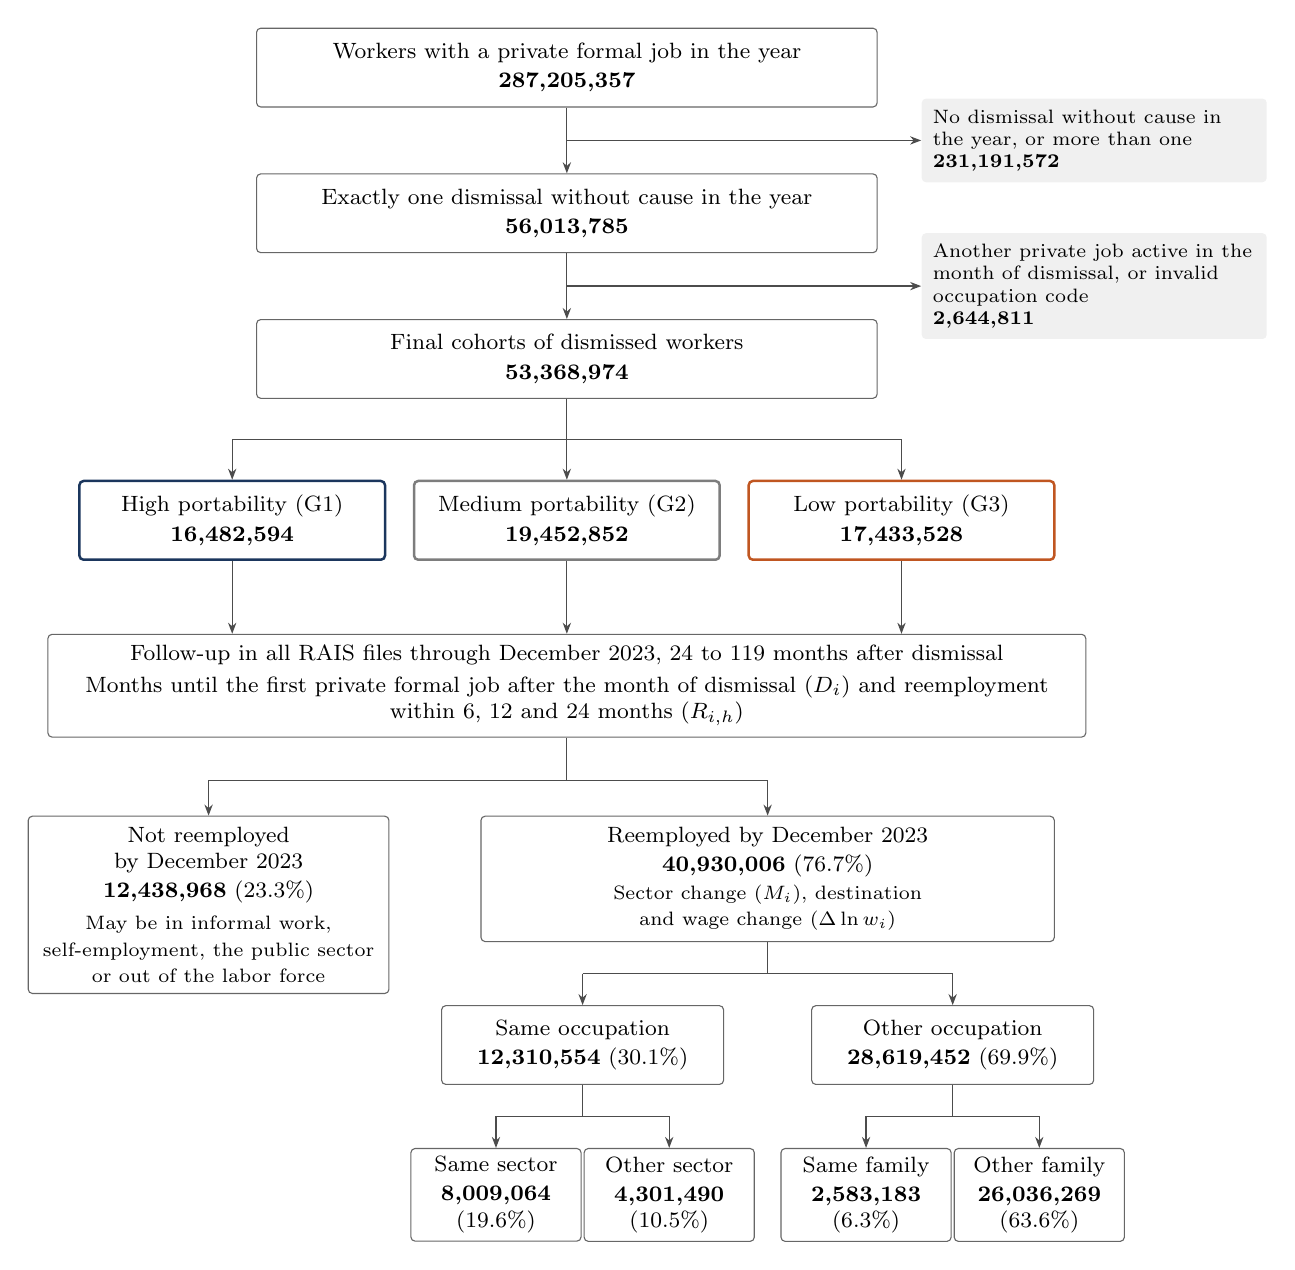
\begin{tikzpicture}[
  font=\footnotesize,
  caixa/.style={draw=black!60, line width=0.4pt, rounded corners=1.5pt,
                align=flush center, inner sep=4pt, minimum height=1.0cm},
  principal/.style={caixa, text width=7.6cm},
  exclui/.style={caixa, draw=none, fill=black!6, text width=4.1cm, align=flush left,
                 font=\scriptsize, minimum height=0.9cm},
  grupo/.style={caixa, text width=3.6cm, line width=0.9pt},
  destino/.style={caixa, text width=3.3cm},
  folha/.style={caixa, text width=1.95cm, inner sep=3pt},
  liga/.style={line width=0.45pt, black!70},
  seta/.style={liga, -{Stealth[length=4pt, width=3pt]}},
]
% ---------------------------------------------------------------- selecao
\node[principal] (A) at (0,0)
  {Workers with a private formal job in the year\\[1pt]\textbf{287,205,357}};
\node[principal] (B) at (0,-1.85)
  {Exactly one dismissal without cause in the year\\[1pt]\textbf{56,013,785}};
\node[principal] (C) at (0,-3.7)
  {Final cohorts of dismissed workers\\[1pt]\textbf{53,368,974}};
\draw[seta] (A) -- (B);
\draw[seta] (B) -- (C);
\node[exclui, anchor=west] (E1) at (4.5,-0.925)
  {No dismissal without cause in the year, or more than one\\\textbf{231,191,572}};
\node[exclui, anchor=west] (E2) at (4.5,-2.775)
  {Another private job active in the month of dismissal, or invalid occupation code\\\textbf{2,644,811}};
\draw[seta] (0,-0.925) -- (E1.west);
\draw[seta] (0,-2.775) -- (E2.west);

% ---------------------------------------------------------------- grupos
\node[grupo, draw=cg1] (G1) at (-4.25,-5.75) {High portability (G1)\\[1pt]\textbf{16,482,594}};
\node[grupo, draw=cg2] (G2) at (0,-5.75)    {Medium portability (G2)\\[1pt]\textbf{19,452,852}};
\node[grupo, draw=cg3] (G3) at (4.25,-5.75)  {Low portability (G3)\\[1pt]\textbf{17,433,528}};
\draw[liga] (C.south) -- (0,-4.72);
\draw[liga] (-4.25,-4.72) -- (4.25,-4.72);
\foreach \g in {G1,G2,G3} \draw[seta] (\g.north |- 0,-4.72) -- (\g.north);

% ---------------------------------------------------------------- acompanhamento
\node[caixa, text width=12.9cm] (F) at (0,-7.85)
  {Follow-up in all RAIS files through December 2023, 24 to 119 months after dismissal\\[2pt]
   Months until the first private formal job after the month of dismissal ($D_i$) and
   reemployment within 6, 12 and 24 months ($R_{i,h}$)};
\foreach \g in {G1,G2,G3} \draw[seta] (\g.south) -- (\g.south |- F.north);

\node[caixa, text width=4.3cm, anchor=north] (N) at (-4.55,-9.5)
  {Not reemployed\\by December 2023\\[1pt]\textbf{12,438,968} (23.3\%)\\[2pt]
   {\scriptsize May be in informal work, self-employment, the public sector or out of the labor force}};
\node[caixa, text width=7.0cm, anchor=north] (R) at (2.55,-9.5)
  {Reemployed by December 2023\\[1pt]\textbf{40,930,006} (76.7\%)\\[2pt]
   {\scriptsize Sector change ($M_i$), destination\\and wage change ($\Delta \ln w_i$)}};
\draw[liga] (F.south) -- (0,-9.05);
\draw[liga] (-4.55,-9.05) -- (2.55,-9.05);
\draw[seta] (-4.55,-9.05) -- (N.north);
\draw[seta] (2.55,-9.05) -- (R.north);

% ---------------------------------------------------------------- destino
\path (R.south) ++(0,-0.4) coordinate (r1);
\node[destino, anchor=north] (O1) at ($(0.2,0)+(0,0 |- r1)+(0,-0.4)$) {Same occupation\\[1pt]\textbf{12,310,554} (30.1\%)};
\node[destino, anchor=north] (O2) at ($(4.9,0)+(0,0 |- r1)+(0,-0.4)$) {Other occupation\\[1pt]\textbf{28,619,452} (69.9\%)};
\draw[liga] (R.south) -- (r1);
\draw[liga] (0.2,0 |- r1) -- (4.9,0 |- r1);
\draw[seta] (0.2,0 |- r1) -- (O1.north);
\draw[seta] (4.9,0 |- r1) -- (O2.north);

\path (O1.south) ++(0,-0.4) coordinate (o1);
\node[folha, anchor=north] (S1) at ($(-0.9,0)+(0,0 |- o1)+(0,-0.4)$) {Same sector\\[1pt]\textbf{8,009,064}\\(19.6\%)};
\node[folha, anchor=north] (S2) at ($(1.3,0)+(0,0 |- o1)+(0,-0.4)$)  {Other sector\\[1pt]\textbf{4,301,490}\\(10.5\%)};
\node[folha, anchor=north] (S3) at ($(3.8,0)+(0,0 |- o1)+(0,-0.4)$)  {Same family\\[1pt]\textbf{2,583,183}\\(6.3\%)};
\node[folha, anchor=north] (S4) at ($(6.0,0)+(0,0 |- o1)+(0,-0.4)$)  {Other family\\[1pt]\textbf{26,036,269}\\(63.6\%)};
\draw[liga] (O1.south) -- (O1.south |- o1);
\draw[liga] (-0.9,0 |- o1) -- (1.3,0 |- o1);
\draw[seta] (-0.9,0 |- o1) -- (S1.north);
\draw[seta] (1.3,0 |- o1) -- (S2.north);
\draw[liga] (O2.south) -- (O2.south |- o1);
\draw[liga] (3.8,0 |- o1) -- (6.0,0 |- o1);
\draw[seta] (3.8,0 |- o1) -- (S3.north);
\draw[seta] (6.0,0 |- o1) -- (S4.north);
\end{tikzpicture}
\end{document}
